\documentclass[a4paper, 12pt]{article}
\usepackage{outlines}
\usepackage{graphicx}
%\usepackage{times}
\usepackage{xcolor}
\usepackage{float}
\usepackage{mathtools}
\usepackage{enumerate}
\usepackage{geometry}
\usepackage[english]{babel}
\usepackage{array}
\usepackage{wrapfig}
\usepackage{amsmath}
\usepackage{multirow}
\usepackage{tabulary}
\usepackage{titlesec}
\usepackage{titletoc}
\usepackage{array}
\usepackage{tabularx,ragged2e,booktabs,caption}
\usepackage{chngcntr}
\usepackage{pgf-pie} 
\usepackage{colortbl} 


\counterwithin{figure}{section}
\counterwithin{table}{section}

\titleformat{\section}[display]%
{\null\fontsize{16}{5}\rmfamily\bfseries\filcenter}{CAPITOLUL \thesection}{1em}{}[]
\titleformat{name = \section, numberless}[block]%
{\null\fontsize{16}{5}\rmfamily\bfseries\filcenter}{}{1em}{}
\titlespacing*{\section}{0em}{1em}{1em}

\titlecontents{section}
[7em] % ie, width of contentslabel + 0.5em
{\medskip}
{\contentslabel[\MakeUppercase\chaptername~\thecontentslabel]{7.5em}}%\thecontentslabel
{\hspace*{-6.5em}}
{\titlerule*[0.5pc]{.}\contentspage}

\addto{\captionsenglish}{
	\renewcommand{\refname}{Referințe bibliografice}%
	\renewcommand{\contentsname}{Cuprins}
	\renewcommand{\listfigurename}{Lista imaginilor}
	\renewcommand{\listtablename}{Lista tabelelor}
}
\addto\captionsenglish{\renewcommand{\chaptername}{Capitolul}}
%define the page geometry
\geometry{
	a4paper,
	left=25mm,
	top=25mm,
	bottom=25mm,
	right=25mm,
}
\renewcommand{\baselinestretch}{1.5}
\makeatletter
\renewcommand\paragraph{\@startsection{paragraph}{4}{\z@}%
	{-2.5ex\@plus -1ex \@minus -.25ex}%
	{1.25ex \@plus .25ex}%
	{\normalfont\normalsize\bfseries}}
\makeatother
\setcounter{secnumdepth}{4} % how many sectioning levels to assign numbers to
\setcounter{tocdepth}{4}    % how many sectioning levels to show in ToC

\begin{document}

%define the title page
\begin{titlepage}
	\begin{center}
		\vspace{0.5cm}
		\large {UNIVERSITATEA "BABEȘ-BOLYAI" CLUJ-NAPOCA}
		
		\large {FACULTATEA DE STUDII EUROPENE}
		\\
		
		
		\vspace{6cm}
		
		\Huge \textbf{LUCRARE DE DISERTAȚIE}
		
		\vspace{2 cm}
		
		\vfill
	\end{center}
	
	\begin{flushleft}
		\large{\textit{Coordonator științific:}} \\
		\large{Conf. univ. dr. Nicoleta Dorina Racolța-Paina}
	\end{flushleft}
	
	\begin{flushright}
		\hfill \large {\textit{Absolvent:}} \\
		\hfill \large {Sorina-Elena Ciucanu}
	\end{flushright}
	
	\begin{center}
		\vspace{1.5cm}
		\large \textbf{2023}
	\end{center}
\end{titlepage}
\begin{titlepage}
	\begin{center}
		\vspace{0.5cm}
		\large {UNIVERSITATEA "BABEȘ-BOLYAI" CLUJ-NAPOCA}
		\\
		\large {FACULTATEA DE STUDII EUROPENE}
		\\\large {SPECIALIZAREA MANAGEMENT PERFORMANT}
		
		\vspace{2.75cm}
		
	
		\huge Abilitățile leaderilor de echipă - de la teorie la practica. 
		
		\huge O cercetare cantitativa  in domeniul IT
		\vspace{1.5 cm}
		
		\vfill
	\end{center}
	
	\begin{flushleft}
		\large{\textit{Coordonator științific:}} \\
		\large{Conf. univ. dr. Nicoleta Dorina Racolța-Paina}
	\end{flushleft}
	
	\begin{flushright}
		\hfill \large {\textit{Absolvent:}} \\
		\hfill \large {Sorina-Elena Ciucanu}
	\end{flushright}
	
	\begin{center}
		\vspace{1.5cm}
		\Large{Cluj Napoca}
		
		\large \textbf{2023}
	\end{center}
\end{titlepage}
\restoregeometry
\thispagestyle{empty}
\section*{Declarație}
\bigskip
\qquad Prin prezenta declar că Lucrarea de disertatie cu titlul "Studiu de caz" este scrisă de mine şi nu a mai fost prezentată niciodată la o altă facultate sau instituţie de învăţământ superior din ţară sau străinătate. De asemenea, declar că toate sursele utilizate, inclusive cele de pe Internet, sunt indicate în lucrare, cu respectarea regulilor de evitare a plagiatului:
	\begin{enumerate}[-]
	\item toate fragmentele de text reproduse exact, chiar şi în traducere proprie din altă limbă, sunt scrise între ghilimele şi deţin referinţa precisă a sursei;
	\item reformularea în cuvinte proprii a textelor scrise de către alţi autori deţine referinţa precisă;
	\item rezumarea ideilor altor autori deţine referinţa precisă la textul original.
	\end{enumerate}

\vspace{3 cm}
\begin{flushleft}
	\large Cluj Napoca,
\end{flushleft}


\begin{flushright}
	\hfill \large Absolvent \textit{Sorina-Elena Ciucanu} \\
	\hfill \large {(semnătura olograf)}
\end{flushright}
\newpage
\thispagestyle{empty}
%put the table of contents
\tableofcontents
\thispagestyle{empty}
%put the list of figures
\newpage
\thispagestyle{empty}
\listoffigures
\newpage
\thispagestyle{empty}
\listoftables


%this section is on new page
\newpage
%\nocite{morgeson2010leadership}



	\section*{Introducere}
\addcontentsline{toc}{section}{\textsc{Introducere}}

\newpage
	\setcounter{section}{0}
	\section{Liderul de echipă în organizațiile contemporane}
\quad \quad\space Într-un context dinamic și competitiv, în care eficiența colaborării și coordonarea echipelor devin din ce în ce mai vitale, liderul echipei (Team Leader) ocupă o poziție centrală în asigurarea succesului și performanței acestora. Prin abilitățile și competențele sale, liderul echipei este capabil să alinieze și să dirijeze echipa spre atingerea obiectivelor organizației. Capitolul următor are ca scop investigarea rolului liderului echipei și a importanței abilităților sale, ce joacă un rol esențial atât la nivelul echipei, cât și la nivelul organizației.
		\subsection{ Team leader - oportunități și provocări}

\quad\quad\space În spatele oricărei organizații de succes se află persoane care își iau un angajament față de misiunea acesteia și care conduc alte grupuri de persoane pentru a fi siguri că acțiunile lor conduc la dezvoltarea și creșterea organică a organizației. Una dintre aceste persoane este liderul de echipă și înainte de a analiza despre activitatea și responsabilitățile acestuia este important să adoptăm o definiție clară a acestui concept. Există mai multe definiții ale liderului de echipă, însă în cadrul acestei lucrări ne vom concentra pe definiția dată de dicționarul de Afaceri Cambridge și anume că " team leader-ul  este persoana responsabilă de o echipă".\footnote{Cambridge Business English Dictionary, meaning of team leader in English.} Prin această afirmație se înțelege că liderul de echipă poartă o responsabilitate fundamentală pentru performanța echipei și acționează ca punct central pentru luarea deciziilor, având ca obiectiv principal atingerea obiectivelor organizației.

	\quad\quad Un alt jucător important în succesul unei organizații,care este deseori confundat cu team leader-ul, este managerul. Cu toate că managerii și liderii de echipă sunt implicați în procese de conducere și coordonare, există diferențe semnificative între abordarea și responsabilitățile acestor două roluri. Astfel, pentru a evidenția rolul unui lider de echipa într-o organizație vom face o comparație a caracteristicilor distinctive ale celor doi, evidențiind contribuțiile și impactul fiecăruia în cadrul organizațiilor.\footnote{What is the difference between a leader and a manager?, https://www.roberthalf.jp/en/management-advice/leadership/leader, accesat in data de 21 mai 2023}
\newpage

	\begin{enumerate}[A)]

		\item\textbf{Definirea rolului în organizație}
		
		\quad Managerul ocupă un rol esential în organizație, având sarcina de a planifica, organiza și controla activitățile echipei și de a asigura eficiența și rentabilitatea. El se implică în delegarea sarcinilor, monitorizarea performanței angajaților și aplicarea politicilor și procedurilor organizației. Pe de altă parte, liderul de echipă are capacitatea de a motiva și ghida membrii echipei în atingerea obiectivelor, creând un mediu de lucru pozitiv și stimulant. Acesta promovează dezvoltarea personală și profesională a angajaților, cultivând colaborarea, comunicarea și creativitatea.
%\footnote{What is the difference between a leader and a manager?, https://www.roberthalf.jp/en/management-advice/leadership/leader, accesat in data de 21 mai 2023}

		\item \textbf{Obiective și priorități}

		\quad\quad Managerii se concentrează pe atingerea obiectivelor organizaționale, planificând și organizând activitățile în concordanță cu acestea. Ei se axează pe rezultate și eficiență, asigurând utilizarea optimă a resurselor. În schimb, team leaders se preocupă de dezvoltarea și motivarea membrilor echipei. Ei își asumă rolul de a inspira și a motiva, promovând colaborarea și încurajând angajații să-și atingă obiectivele individuale și să contribuie la succesul colectiv. Astfel, managerii urmăresc realizarea obiectivelor organizației, în timp ce liderii de echipă se concentrează pe creșterea și dezvoltarea personală a membrilor echipei.

		\item \textbf{Abordarea comunicării}
		
		\quad\quad Managerii utilizează comunicarea formală și directivă pentru a transmite instrucțiuni și a asigura respectarea regulilor și politicii organizației. Ei se concentrează pe îndeplinirea sarcinilor și atingerea obiectivelor. În schimb, liderii de echipă adoptă o abordare mai deschisă și empatică în comunicare, ascultând și implicând membrii echipei în procesul decizional. Ei promovează schimbul de idei și feedback constructiv pentru a încuraja colaborarea și participarea activă a membrilor echipei.

		\item \textbf{Gestionarea conflictelor}

		\quad\quad Managerii utilizează reguli și proceduri pentru a gestiona conflictele și a menține stabilitatea în echipă, în timp ce liderii de echipă văd conflictele ca o oportunitate de creștere și promovează dialogul deschis și rezolvarea constructivă. Managerii se concentrează pe rezolvarea eficientă a conflictelor, în timp ce liderii încurajează membrii echipei să-și exprime punctele de vedere și să găsească soluții comune. Astfel, abordarea conflictelor diferă între manageri și lideri de echipă, având în vedere prioritățile și perspectivele lor distincte.

		\item \textbf{Delegarea autorității}

		\quad\quad Managerii delegă sarcini și responsabilități pentru a coordona și monitoriza activitatea echipei în vederea atingerii obiectivelor organizaționale, în timp ce liderii de echipă utilizează delegarea pentru a stimula dezvoltarea și creșterea individuală. Managerii se concentrează pe eficiența operațională, în timp ce liderii încurajează membrii echipei să-și asume roluri de lider și să-și valorifice potențialul. Astfel, abordarea delegării diferă între manageri și lideri, având în vedere scopurile și perspectivele lor specifice.

	\end{enumerate}

	%\quad Chiar daca exista diferente intre cei doi managerii și liderii de echipă reprezinta două roluri esențiale în contextul organizațional actual. În timp ce managerii se concentrează mai mult pe coordonarea activităților și atingerea obiectivelor organizaționale, liderii de echipă își ghidează și motivează angajații către succes prin intermediul comunicării, inspirației și dezvoltării personale. Pentru a obține rezultate optime, organizațiile trebuie să recunoască importanța ambelor roluri și să cultive atât abilități manageriale, cât și abilități de leadership în interiorul echipei.

	\quad\space Alături de toate aceste caracteristici pe care le-am evidențiat anterior, o parte importantă din rolul unui team leader se referă la acțiunile pe care le întreprinde în cadrul echipei pentru a asigura coordonarea și succesul acesteia. Activitatea principala implică gestionarea unei echipe, asigurându-se că obiectivele sunt atinse în mod eficient, în același timp fiind responsabili de planificarea și organizarea activităților, delegarea sarcinilor, motivarea membrilor echipei și menținerea unei colaborări cât mai productive. Conform studiului realizat de Frederick P. Morgeson și a colaboratorilor, din anul 2010, asupra proceselor de leadership \footnote{Frederick P. Morgeson, D. Scott DeRue, Elizabeth P. Karam, Leadership în Teams: A Funcțional Approach to Understanding Leadership Structures and Processes,2010}, putem clasifică activitățile unui team leader în două faze: 
	\begin{itemize}

	\item \textbf{Faza de tranziție}: în care echipele se concentrează asupra activităților legate de structurarea echipei, planificarea lucrului echipei și evaluarea performanței echipei, astfel încât echipa să poată atinge în cele din urmă obiectivul sau scopul său. În timpul acestei perioade  se enumera activitati precum asigurarea unei combinații potrivite de persoane în echipă, definirea misiunii generale, a obiectivelor și a standardelor de performanță ale echipei, structurarea rolurilor și responsabilităților în echipăm, asigurarea ca toți membrii echipei să fie capabili să performeze eficient, înțelegerea mediului echipei si facilitarea proceselor de feedback în echipă. 

	\item \textbf{Faza de acțiune}: care include porțiunea ciclului de performanță a echipei unde se concentrează pe activități care contribuie direct la atingerea obiectivelor sale. In timpul acestei faze se exercită actiuni precum monitorizarea echipei și a mediului său de performanță, gestionarea granițelor dintre echipă și mediul organizațional mai larg, provocarea echipei să se îmbunătățească în mod continuu, implicarea în efectuarea activităților echipei, rezolvarea problemelor cu care echipa se confruntă, obținerea resurselor pentru echipă, încurajarea echipei să acționeze autonom și cultivarea unui climat social pozitiv în cadrul echipei. 
	\end{itemize}

\quad\space 

%\quad\quad\space Tipuri de lideri- teorie vs practica?? 


	\quad\space Un pilon fundamental al succesului organizațional, care reprezinta totodată și instrumentul de baza a unui team leader, este echipa. Echipa este un grup de indivizi care îndeplinesc roluri specifice și interacționează dinamic, interdependent și adaptabil în vederea atingerii unui obiectiv comun. \footnote{Denise L. Reyes, Julie Dinh, Eduardo Sălaș, What Makes A Good Leader?, 2019} Echipele contemporane necesită mai multă atenție și interacțiune continuă pentru a menține o performanță ridicată pe parcursul vieții lor temporare. Team leader-ul trebuie acum să se concentreze pe motivarea și susținerea echipelor personalizând procesul în funcție de membrii echipei. Luând în considerare articolul lui Victor Sohmen,despre leadership și teamwork\footnote{ Victor Sohmen, Leadership and teamwork: Two sides of the same coin, 2013}, se pot constata opt aspecte esențiale care facilitează legătură dintre team leader și lucrul în echipa.
	\begin{itemize}
	\item\textbf{Viziunea} este primul element pe care orice lider ar trebui să împărtășească de la început cu echipa sa. Prin implicarea membrilor echipei în dezvoltarea viziunii și asigurând o aliniere constantă cu obiectivele organizației, liderul creează un sentiment de apartenență și împuternicire în echipă.

	\item Un alt element important este \textbf{integritatea} care generează încredere, respect și credibilitate membrilor echipei față de acțiunile pe care le întreprinde liderul.

	\item \textbf{Comunicarea} este alt aspect important deoarece team leader-ul reprezintă legătură echipei cu organizația. Acesta trebuie să comunice clar obiectivele, responsabilitățile, gradul de perfomanță, nivelul de așteptări și modul de a oferi feedback.

	\item Un detaliu ce nu poate lipsi dintr-o echipă este \textbf{colaborarea}. Liderii de succes se adaptează în funcție de situație și crează un mediu propice în care fiecare membru al echipei are un rol bine stabilit și oferă un plus de valoare.

	\item \textbf{Orientarea către obiective} este un alt element ce are un impact mare asupra activităților unui lider. Pe toată perioada colaborării team leader-ul trebuie să țină cont de obiectivele organizației și să le îmbine cu obiectivele personale ale membrilor echipei. Prin implicarea comună în atingerea acestor obiective se consolidează colaborarea și succesul echipei.

	\item Un element nou este \textbf{empowermentul} care înseamnă dezvoltarea încrederii de sine și autonomie în membrii echipei. Acest lucru poate avea loc prin comunicare eficientă între team leader și team members, prin delegarea responsabilităților la persoanele potrivite și prin ședințe de mentorat și poate contribui la construirea unor relații pozitive și la realizarea obiectivelor echipei. 

	\item Un alt aspect ce poate fi folosit de către team leader este \textbf{creativitatea} care poate fi un avantaj dacă este utilizată în mod constructiv. Prin promovarea unui mediu de lucru sănătos care încurajează inovația, liderii pot îmbunătăți și transforma rezultatele organizației, astfel încât să obțină un avantaj competitiv pe piață existentă. 

	\item Ultimul element pe care s-a pus tot mai mare accentul în ultima perioada este\textbf{ team-building-ul}. Echipa începe ca un grup de străini și trebuie să fie sinergizată într-o echipa de înaltă performanță, iar liderul de echipa are un rol semnificativ în definirea atmosferei de la locul de muncă. Echipa trebuie să fie dezvoltată într-un mod care să promoveze o cultură pozitivă de construire a echipei. 

	\end{itemize}

	\quad În contextul managementului echipei, dobândirea și dezvoltarea abilităților de leadership reprezintă un aspect crucial pentru obținerea succesului insa conducerea eficientă a unei echipe nu necesită doar competențe tehnice și experiență, ci și înțelegerea profunzimii rolului de lider si aplicarea autoritatii intr-un mod cat mai echilibrat. Astfel, potrivit unui articol scris de Dr. Radhika Kapur\footnote{Dr. Radhika Kapur,Leadership Skills: Fundamental in Leading to Effective Functioning of the Organizations, 2020} , se evidențiază trei trăsături importante pe care un lider trebuie să le dețină pentru a atinge succesul, și anume:

	\begin{itemize}
	\item \textbf {Dorința de a conduce} este crucială pentru a furniza cunoștințe, motivație și soluții, promovând astfel succesul și dezvoltarea organizațională. Fără a avea motivația intrinsecă de a conduce liderul va ajunge să aibă o rezistență față de munca de conducere iar membrii echipei vor resimți acest lucru și nu va mai exista o colaborare eficientă.

	 \item \textbf{Angajamentul față de misiunea și viziunea organizației} facilitează generarea unei conștientizări în ceea ce privește metodele, abordările și strategiile care vor fi puse în practică pentru a asigura funcționarea eficientă a organizației și realizarea misiunii și a obiectivelor. Misiunea și viziunea se concentrează în principal asupra a ceea ce va face organizația, cui îi va servi și cum obiectivele și funcționarea organizației vor fi benefice comunității. 

	 \item\textbf{Integritatea} este o trasatură de care liderii pot beneficia în numeroase moduri. Acestea includ îndeplinirea eficientă a responsabilităților de serviciu, formarea unor relații cordiale cu ceilalți, obținerea respectului și aprecierii, capacitatea de a lucra sub stres, abilitatea de a face față problemelor și provocărilor, precizia în îndeplinirea sarcinilor de serviciu, onestitatea și dreptatea și tratarea cu respect și politețe a celorlalți indivizi, atât interni, cât și externi organizației. Acești factori sunt benefici pentru membrii echipei și pentru organizație în ansamblu. 

\end{itemize}

	\space\quad\quad  În societatea actuală, în care evoluția și schimbarea sunt inevitabile, dezvoltarea continuă a devenit un aspect esențial pentru atingerea succesului personal și profesional. Ideea de a căuta și de a adopta o abordare orientată spre dezvoltare a devenit din ce în ce mai importantă într-o lume în care cunoștințele și competențele se depreciază rapid. La fel se întâmplă și în cazul liderilor de echipă care se confruntă zilnic cu noi tendințe și provocări apărute pe piața muncii. Trăind într-o eră a tehnologiei, accesul la informații nu a fost niciodată mai facil, iar sursele de îmbunătățire se află la un click distanță. În conformitate cu cercetarea efectuată de Radhika Kapur ibidem (2020)\footnote{Ibidem}, s-au evidențiat câteva obiceiuri care pot ajută liderii de echipa să-și îmbunătățească rolul pe care îl dețin. Printre ele se enumeră:
	
	\begin{itemize}

	\item\textbf{ Dezvoltarea pasiunii} este esentiala pentru imbunatatirea abilitatilor de conducere. Aceasta îi ajută să-și îndeplinească responsabilitățile cu pasiune și să obțină rezultatele dorite.Pe lângă beneficiile personale, dezvoltarea pasiunii în lideri are și un impact asupra subordonaților lor deoarece pot transmite entuziasm și inspirație celor din jurul lor, creând un mediu de lucru pozitiv și motivant. De asemenea, pasiunea dezvoltată în lideri îi ajută să facă față cu succes provocărilor și obstacolelor pe care le întâlnesc în activitatea lor. Fiind pasionați, aceștia sunt mai puțin predispuși la descurajare și  sa renunțe în fața dificultăților. În schimb, pasiunea îi încurajează să caute soluții creative și să găsească modalități inovatoare de a depăși obstacolele.

	\item Liderii trebuie să \textbf{recompenseze și să motiveze} angajații pentru a îmbunătăți abilitățile de leadership. Prin oferirea de recompense și stimulente, precum și prin promovarea și concediile plătite, angajații devin mai interesați și entuziasmați în îndeplinirea sarcinilor lor de serviciu. Această motivație ajută la concentrarea și angajamentul angajaților în atingerea obiectivelor organizației. Această abordare este considerată unul dintre modurile cruciale de a stimula concentrarea și angajamentul angajaților față de îndeplinirea sarcinilor de serviciu.

	\item Liderii trebuie să se angajeze în \textbf{cercetare periodică}, utilizând diverse surse precum internetul, cărți și articole, pentru a-și îmbunătăți abilitățile de leadership. Această cercetare poate include și implicarea în lucrări de teren, oferindu-le liderilor informații practice și experiențe relevante. Prin utilizarea tehnologiei și internetului, liderii pot accesa numeroase resurse și studii despre modalități de a-și îmbunătăți abilitățile de leadership.


	\item În interiorul organizațiilor, angajații se confruntă cu diverse probleme legate de sarcinile și responsabilitățile de serviciu, infrastructură, facilități, resurse și condiții de lucru. Pentru a aborda aceste probleme, este necesară \textbf{implementarea unui sistem eficient de soluționare a reclamațiilor}, care să permită angajaților să-și exprime nemulțumirile și să primească soluții adecvate. Prin asigurarea unui astfel de sistem, liderii pot promova satisfacția angajaților și pot contribui la îmbunătățirea abilităților lor de leadership.

	\item \textbf{Conștientizarea situațională} implică percepția elementelor și evenimentelor din mediu în raport cu timpul și spațiul (A Practical Guide to Situational Awareness, 2012). Liderii integrează avansurile tehnologice în sarcinile lor și folosesc metode moderne de învățare în programele de pregătire. Dezvoltarea conștientizării situaționale este esențială pentru a face față cu succes condițiilor de mediu interne și externe. 

	\end{itemize}

	\subsection{Abilități și competențe specifice team leader-ului}
	
	\quad\quad În fiecare organizație, indiferent de mărimea acesteia, există diverse categorii de lideri. În literatura de specialitate, se menționează prezența a două feluri principale de lideri și anume: informali, exercitând o influență semnificativă asupra colegilor datorită personalității și calităților sale și formali, ocupând o poziție oficială cu putere și autoritate de a lua decizii , însă ambele tipuri împărtășesc abilități care îi ajută să atingă obiectivele personale sau ale organizației. Aceste abilități de leadership pot fi considerate instrumente, comportamente și capacități esențiale pentru a promova bunăstarea angajaților și a îmbunătăți performanța organizației.\footnote{MTD Training, Leadership Skills, 2010} Indiferent de poziția lor, liderii își focalizează eforturile în direcționarea și motivarea angajaților pentru a atinge sarcinile și obiectivele stabilite. Prin dezvoltarea potențialului individual al celorlalți, liderii autentici demonstrează o abilitate de leadership remarcabilă. Pentru a avea succes în implementarea acestor abilități, liderii trebuie să faciliteze dezvoltarea competențelor celorlalți, adaptându-se la diverse situații și asigurând beneficii atât pentru angajați, cât și pentru organizație.

	\quad  Un detaliu ce ar trebui menționat în interiorul acestui subcapitol este deosebirea dintre abilități și competențe. Chiar dacă limitele dintre ele pot fi neclare și pot varia în funcție de contextul utilizat între ele există o diferența. Pe de o parte abilitățile sunt aptitudini practice și specifice unei persoane de a execută anumite activități sau sarcini. Ele pot fi dobândite și dezvoltate prin experiență, învățare și antrenament. Exemple de abilități includ capacitatea de a comunica eficient, de a rezolva probleme, de a lucra în echipă sau de a utiliza tehnologii specifice. Pe de altă parte competențele sunt mai complexe și implică o combinație de cunoștințe, abilități și atitudini. Ele reflectă capacitatea unei persoane de a-și aplică abilitățile într-un context specific și de a obține rezultate de calitate într-o anumită arie de activitate. Competențele pot include capacitatea de a lua decizii înțelepte, de a rezolva probleme complexe, de a lidera și de a influența oamenii, de a gestiona proiecte sau de a gândi strategic.\footnote{Skills and Competencies: What’s the Difference?, 2022,https://blog.degreed.com/skills-and-competencies/, accesat la data de 21 mai 2023}
		
	\quad\quad Noile schimbari in era tehnologiei au intensificat necesitatea unor lideri cu o perspectivă multidimensională, capabili să gestioneze diversitatea de acțiuni necesare pentru implementarea planului strategic. Complexitatea mediului a sporit considerabil așteptările părților interesate, depășind sfera evidentului. Astfel, liderii din zilele noastre sunt așteptați să fie deplin competenți și pregătiți să abordeze riscurile atât cunoscute, cât și necunoscute. In urma cercetarilor efectuate de Victor Sohmen, de la Drexel University, in anul 2013, s-a remarcat "modelul Competentelor de leadership" impartit pe cinci dimensiuni in care sunt sintetizate competentele ce sunt necesare oricarui lider de echipa.\footnote {Victor Sohmen, Leadership and teamwork: Two sides of the same coin, 2013}

	\begin{enumerate}[(1)]

		\item Liderii \textbf {transformationali}  sunt indivizi carismatici care au capacitatea de a influența și mobiliza o echipă pentru a atinge obiectivele strategice ale organizației. Ei promovează o cultură bazată pe integritate, transparență și respect autentic, inspirând urmăritorii să depășească așteptările și construind relații de lucru sănătoase. Prin aceasta, se creează o atmosferă de împuternicire și entuziasm vizibil în realizarea obiectivelor.

		\item Liderii \textbf {tranzacționali} stabilesc o relație de lucru bazată pe tranzacții, oferind recompense tangibile și intangibile în schimbul îndeplinirii sarcinilor. Ei comunică obiectivele strategice și motivează echipa prin asocierea performanței ridicate cu recompense valoroase. Această abordare a leadership-ului tranzacțional contribuie la formarea și menținerea unei echipe unite și cu rezultate pozitive.

		\item Leadershipul \textbf {organic} facilitează interacțiunea intensă și consolidează relațiile de lucru în cadrul echipei. Prin promovarea unei viziuni și a valorilor comune, liderul împuternicește și îndrumă membrii motivați ai echipei pentru a-și dezvolta abilitățile de leadership proprii.
		
		\item Liderii \textbf{contemporani}  adoptă o abordare democratică, folosind influență și persuasiune în locul fricii pentru a conduce echipa. Ei gestionează ambiguitatea și paradoxul, echilibrând schimbarea cu stabilitatea, viziunea cu obiectivele și inovarea cu conformitatea, pentru a îndeplini obiectivele strategice ale organizației și așteptările părților interesate.

		\item Liderii \textbf{etici} sunt modele de integritate care inspiră respect și admiratie în rândul echipei și părților interesate. Leadershipul etic se axează pe utilizarea responsabilă a puterii sociale în luarea deciziilor, acțiunilor întreprinse și influențarea celorlalți (Resick, Hanges, Dickson, Mitchelson, 2006, p. 346). Prin promovarea valorilor și practicilor etice, liderul devine un exemplu inestimabil, atât pentru organizație, cât și pentru membrii echipei.

	\end{enumerate}

	%\quad\quad Perioada de epidemie și izolare din 2020 a determinat multe companii din sectorul public și privat să adopte lucrul la distanță. În acest context, tehnologiile digitale au jucat un rol esential în transformarea modului de conducere și în crearea unor noi modalități de comunicare și colaborare virtuală intre team leader si echipa. Astfel, in urma acestei transformari s-a creat un nou concept care a marcat modul in care liderii si membrii echipei se raporteaza unul la celalalt in cadrul organizatiilor si anume termenul de E-leader (lider electronic) sau E-leadership. E-leaderii au fost nevoiti sa-si completeze pachetul de abilitati pentru a gestiona divese platforme de comunicare dar si sa se adapteze la noile cerinte. In acest sens,una din noile cerinte a fost ca  liderii electronici  sa dezvolte competente interculturarale pentru a comunica adecvat cu membrii echipei si pentru a intelege diferentele si asemanarile dintre culturile acestora. Aceasta provocare i-a determinat pe lideri sa dezvolte noi competente  avand in vedere noile structuri de lucru din punct de vedere tehnic dar si abilitati care au pus accent mai mare  asupra relatiei dintre lider si angajat, din punct de vedere social. 

    \quad\quad Perioada de epidemie și izolare din 2020  a determinat multe companii din sectorul public și privat să adopte lucrul la distanță. Acest context a impus utilizarea tehnologiilor digitale, care au jucat un rol cruciall în transformarea modului de conducere și în crearea unor noi modalități de comunicare și colaborare virtuală între liderii de echipă și membrii echipei. Ca rezultat al acestei transformări, a apărut conceptul de E-leader (lider electronic) sau E-leadership\footnote{Francoise Contreras*, Elif Baykal and Ghulam Abid,E-Leadership and Teleworking in Times of COVID-19 and Beyond: What We Know and Where Do We Go, 2020}
 care a marcat modul în care liderii și membrii echipei se raportează unul la celălalt în cadrul organizațiilor din care fac parte. E-leaderii au fost nevoiți să își completeze setul de abilități pentru a gestiona diverse platforme de comunicare și să se adapteze la noile cerințe. În acest sens, o cerință nouă a fost dezvoltarea competențelor interculturale pentru a comunica adecvat cu membrii echipei și pentru a înțelege diferențele și asemănările dintre culturile acestora. Această provocare a determinat team leaders să dezvolte noi competențe, atât din punct de vedere tehnic, în ceea ce privește noile structuri de lucru, cât și din punct de vedere social, accentuând relația dintre lider și angajat.

	\quad În cele din urmă,  realitatea virtuală i-a facut pe oameni mai vulnerabili, iar "abilitățile soft" și inteligența emoțională au devenit cruciale pentru comunicarea online. McCleskey susține că noii lideri vor solicita astfel de abilități care să le permită să facă față provocărilor generate de diversitatea crescută, heterogenitatea grupurilor de lucru, nivelul ridicat de ambiguitate și necesitatea de abordări mai personalizate (McCleskey, 2015).\footnote { Inna Semenets-ORLOVA,Alla Klochko, Tetiana Shkoda, Olena Marusina, Mariia Tepliuk, Emotional Intelligence as the Basis for the Development of Organizational Leadership During the Covid Period (Educational Institution Case), 2021}Conceptul de inteligență emoțională a fost introdus in 1990, de catre J. Mayer și P. Salovey , care au definit-o drept abilitatea de a recunoaște, distinge și gestiona emoțiile proprii și ale altor persoane, utilizându-le în mod eficient pentru a-și controla comportamentul.\footnote{ibidem} 

	\quad\quad Un aspect important legat de inteligența emoțională (IE) este faptul ca se bazează pe autocunoaștere. Astfel un lider cu o stima de sine ridicată poate influența în mod pozitiv relația cu echipa sa și să încurajeze dezvoltarea unei culturi organizaționale bazate pe încredere și respect reciproc. Această abordare promovează o comunicare deschisă și sinceră între lider și membrii echipei, ceea ce facilitează exprimarea liberă a opiniilor și ideilor. În același timp, persoanele cu un nivel ridicat de inteligență emoțională (IE) sunt mai susceptibile să fie conștiente de impactul lor asupra celor din jur și să dezvolte relații mai pozitive în cadrul organizației.

	\quad\quad Un prim pas pe care un lider de echipă îl poate întreprinde în această direcție este să obțină cunoștințe despre opiniile și percepțiile membrilor echipei sale, astfel identificând punctele slabe și punctele forte ale relației de lucru dintre el și membrii echipei. În urma analizei mai multor articole de specialitate, s-a constatat că angajații consideră aceste aspecte ca fiind deosebit de importante în ceea ce privește calitățile unui lider de echipă:
	\begin{itemize}

	\item \textbf {Entuziasmul și pasiunea}  sunt două trăsături esențiale care nu ar trebui să fie neglijate de către un lider, deoarece au un impact semnificativ asupra echipei și clienților săi. Ele sunt contagioase și au capacitatea de a atrage oamenii către lider și de a încuraja participarea activă. În plus, în perioadele dificile, entuziasmul și pasiunea devin și mai importante, oferind energia și determinarea necesare pentru a depăși obstacolele și a menține un sentiment de direcție și scop în cadrul echipei.\footnote{Maria Johnson, Leadership from an employee's perspective, 2017,  https://www.linkedin.com/pulse/leadership-from-employees-perspective-maria-johnson/, accesat in data de 21 mai 2023}
	\item\textbf{Rezistarea sub presiune} este considerată un privilegiu ce este câștigat prin efort și perseverență. Atât în viața personală, cât și în cea profesională, întâlnim diverse provocări și presiuni. Însă modul în care gestionăm această presiune și ne manifestăm autentic în astfel de situații ne definește cu adevărat ca indivizi. Este esențial să putem privi în oglindă și să ne simțim mândri de felul în care am abordat aceste situații și am reușit să ne menținem integritatea.\footnote{ibidem}

	\item \textbf{Curajul de a admite atunci când se comit greșeli sau când nu se cunoaște răspunsul.} Deși s-ar putea presupune că recunoașterea greșelilor sau a lipsei de răspuns poate slăbi încrederea, contrariul este adevărat. Prin recunoașterea sinceră și deschisă a greșelilor, un lider construiește încredere și favorizează un mediu în care toți membrii echipei pot învăța și crește. În plus, atunci când liderul nu posedă răspunsurile necesare, faptul de a recunoaște acest aspect și de a ilustra eforturile depuse pentru a obține informațiile necesare oferă un exemplu pozitiv pentru întreaga echipă.\footnote{Team ClearWater, What Makes a Great Leader: An Employee's Perspective, 2019,https://www.clearwater-consulting.com/blog/what-makes-a-great-leader-an-employees-perspective, accesat la data de 21 mai 2023}

	\item\textbf{Recunoașterea și aprecierea} ocupă un rol esențial în cadrul leadershipului, oferind o motivație eficientă pentru angajați și consolidând încrederea și satisfacția acestora în organizație. Prin oferirea de feedback pozitiv, exprimarea aprecierii și acordarea de recompense tangibile, liderul poate inspira angajații să își depășească limitele și să ofere performanțe remarcabile.\footnote{ibidem}

		\item Acordarea atenției angajaților prin \textbf {ascultarea activă} este un aspect esențial al liderilor, care trebuie să ofere oportunitatea angajaților de a-și exprima opiniile și de a contribui cu idei. Ascultarea atentă și deschiderea către sugestii permit liderilor să beneficieze de aportul valoros al echipei și să promoveze inovația în organizație. Prin implicarea activă a angajaților, se poate crea un mediu de lucru colaborativ și motivant.\footnote{MARIA TANSKI-PHILLIPS ,What Do Employees Want from Their Leaders? 7 Leadership Tips to Follow, 2019, https://smallbusiness.patriotsoftware.com/employees-want-leaders-7-leadership-tips-follow/, accesat in data de 21 mai 2023}
	

	\item Este crucial ca liderul \textbf{ să ofere o viziune clară și bine definită}, deoarece absența acesteia poate dificulta implicarea și angajamentul angajaților. Capacitatea liderului de a exprima cu precizie importanța situației sau a proiectului reprezintă un factor determinant în obținerea aderării și entuziasmului echipelor. Indiferent de natura proiectului, abilitatea de a crea un sentiment de importanță si apartenență contribuie la mobilizarea angajaților pentru atingerea obiectivelor propuse.\footnote{ibidem}

	\end{itemize}

		%\quad Avand in vedere ca traim intr-o lume in continua schimbare si evolutie, angajatii trebuie sa se adapteze de la an la an noilor provocari ce apar pe piata muncii. Apar noi tendinte ce schimba paradigma relatiei dintre sef si subordanat transformandu-se intr-un parteneriat in care ambele parti lucreaza impreuna pentru a atinge succesul. In acest caz, exista 
	\quad\quad Într-un secol al vitezei caracterizat de transformări sociale, tehnologice și economice, adaptabilitatea angajaților la schimbare devine un factor important pentru succesul organizațional. Această dinamică schimbă paradigma relației dintre lider și subordonați, trecând de la un model de autoritate strictă la un parteneriat colaborativ. În acest nou context, liderii de echipă trebuie să își dezvolte și să-și actualizeze abilitățile pentru a se adapta la provocările viitoare și pentru a își ghida eficient echipa în direcția succesului. Se consideră că prin previzionare și pregătire pentru evenimentele viitoare, acești lideri pot asigura un avantaj competitiv și pot anticipa nevoile în continuă schimbare ale organizației. Câteva dintre tendințele ce se preconizează a fi importante până în anul 2030 sunt:

	\begin{itemize}
	\item \textbf{Servant Leadership}\footnote{The Future of Leadership in 2030: 6 New Disruptive Trends, 2022, https://quantic.edu/blog/2022/08/05/the-future-of-leadership-in-2030-6-new-disruptive-trends/, accesat in data de 21 mai 2023} reprezintă un concept viitor în care liderul adoptă valorile unui lider servitor care conduce în scopul satisfacerii nevoilor celorlalți. Această abordare se concentrează pe bunăstarea angajaților și a comunităților lor, în detrimentul prioritizării obiectivelor companiei sau afacerii. Acest tip de leadership se bazează pe implicarea activă a liderului în sprijinirea și dezvoltarea membrilor echipei, promovând o cultură a colaborării și a atenției față de nevoile individuale.

%\quad reprezintă un model viitor în care liderul îmbrățișează valorile unui lider servitor care conduce pentru a satisface nevoile celorlalți. Acesta se concentrează pe bunăstarea forței de muncă și a comunităților acestora. În loc să prioritizeze obiectivele companiei sau afacerii, accentul leadershipului servitor rămâne centrat pe bunăstarea oamenilor săi.


	\item Conform profesorului Ibarra,\footnote{HERMINIA IBARRA, Five leadership skills for the future,2022, https://www.london.edu/think/five-leadership-skills-for-the-future, accesat in data de 21 mai 2023}  un element de viitor este \textbf{coachingul} deoarece se bazează pe împuternicirea individului pentru a-și folosi autonomia într-un mod adaptiv și agil. Acest proces implică adresarea de întrebări adecvate, care să valideze cunoștințele și încrederea angajaților, încurajându-i să-și aducă propria creativitate, gândire inovatoare și soluții în cadrul organizației. Astfel, coachingul promovează o cultură în care liderii se simt încrezători în capacitatea lor de a identifica și rezolva probleme, contribuind atât la dezvoltarea lor personală, cât și la succesul organizațional.

\item \textbf{Abilitățile de ascultare} reprezintă o competență esențială pentru liderii de viitor. Deși comunicarea eficientă este recunoscută ca fiind importantă, se subestimează adesea rolul ascultării active în calitate de lider. În loc să vorbească în nume propriu, liderii viitori acordă importanță ascultării atente și manifestă interes față de perspectiva celorlalți. Prin ascultarea activă a clienților și a angajaților, aceștia pot identifica și elimina obstacolele, oferind sprijin și stimulând motivația pentru a obține succesul în organizație.\footnote{Tony Nutley,Future Leaders: 6 Key Skills Required for Next Gen Leadership, 2022, https://www.linkedin.com/pulse/future-leaders-6-key-skills-required-next-gen-tony-nutley/, accesat in data de 21 mai 2023} 

	\end{itemize}


	\subsection{Munca liderilor în contextul diversităților tipurilor de echipe }

	\quad\quad Pe parcursul ultimelor decenii, activitatea și rolul liderului de echipă au suferit o adaptare constantă pentru a răspunde noilor contexte în evoluție. Această evoluție continuă a dat naștere la o serie de provocări în fiecare zi, care au necesitat abordări și soluții noi. Situația generată de pandemia COVID-19 nu a reprezentat o exceptie de la regulă si a impus tuturor companiilor sa  reactioneze și să adopte un nou stil de lucru intr-un timp foarte scurt. Cateva dintre provocarile pe care le-au intampinat sunt evidentiate in articolul lui Reyes, 2021\footnote{Denise L. Reyes, Miguel Luna, Eduardo Salas, Challenges for team leaders transitioning from face-to-face to virtual teams, 2021} :

	\begin{itemize}

	\item Prima provocare pe care liderii au intampinat-o a fost mentinerea productivitatii angajatilor. In acest sens, au existat doua tendinte pe care membrii echipei le-au urmat in munca lor de acasa. Pe de o parte au fost cei care au intampinat dificultati in a se concentra asupra task-urilor din cauza unor factori perturbatori de acasa precum familia, vecinii si alte responsabilitati dar pe de alta parte au fost cei care au avut dificultăți în a delimita timpul de muncă și a se opri după cele 8 ore de lucru,  fiind tentați să lucreze în mod excesiv.

	\item O alta provocare pe care team leader-ul a fost nevoit sa o rezolve a fost sa se asigure ca membrii echipei se simt conectati atat in echipa cat si in organizatie, . Comunicarea a jucat un rol foarte important in aceasta privinta deoarece lucrand de la distanta, liderul nu mai avea contact fizic/direct cu angajatii ca sa-si dea seama de eventualele probleme cu care s-ar putea confrunta ei sau ce nevoi individuale pot avea la nivel de echipa.

	\item Avand in vedere vulnerabilitatea angajatilor, o noua provocare a fost asigurarea unui mediu in care se promova siguranta psihologica. Liderii au fost nevoiti sa creeze un cadru care sa faciliteze deschiderea si exprimarea libera a ideilor si preocuparilor membrilor echipei, astfel incat sa existe un climat de incredere si respect reciproc intre cele doua parti. 


	\end{itemize}


	\quad\quad In cadrul mediului de lucru, liderul de echipa nu ar putea atinge obiectivele organizatiei daca nu ar avea o echipa care sa-l sustina in acest proces. Odata cu evolutia noilor contexte, echipa a avut si ea de suferit diverse schimbari care au necesitat abordari noi si metodologii diverse. In urmatoarele randuri vom analiza patru tipuri de echipe care există țn prezent și caracteristicile acestora:

%
%\footnote{Denise L. Reyes, et al. What Makes a Good Leader?, 2019}
	\begin{itemize}

	\item \textbf{Echipele Virtuale} sunt echipe ce au membrii care sunt dispersați geografic, dar lucrează împreună într-o sarcină interdependentă prin intermediul mijloacelor electronice, având o interacțiune față în față redusă. Provocarea principala cu care se confrunte membrii dintr-o asemenea echipa este coordonarea sarcinilor in diferite locatii geografice, fusuri orare si culturi. Similar echipelor tradiționale, conducerea unei echipe virtuale necesită abilități de leadership și management. După cum a afirmat Nayani et al. (2018), organizațiile ar trebui să asigure siguranța și sănătatea ocupațională a lucrătorilor la distanță prin intermediul unui management adecvat (adică sisteme, proceduri și practici) și a practicilor de leadership eficiente.\footnote{Francoise Contreras*, Elif Baykal and Ghulam Abid,E-Leadership and Teleworking in Times of COVID-19 and Beyond: What We Know and Where Do We Go, 2020}

	\item \textbf{Echipele} care lucreaza in mod \textbf{hybrid} au o structura flexibila de lucru in care unii angajati lucreaza in mod remote, iar ceilalti membrii de la birou. Echipele hibride nu se conformează unui singur mediu de lucru, deoarece toți angajații lucrează în mod diferit. Prin acest model, organizațiile pot beneficia de o flexibilitate crescută, acces la un piata mai larga de talente și un echilibru mai bun între viața personală și profesională, păstrând în același timp avantajele interacțiunilor față în față și a spațiilor de lucru fizice. \footnote{Miro Miroslavov, Hybrid Team Collaboration: Navigating Best Practices [2023], https://www.officernd.com/blog/hybrid-work/hybrid-workforce-collaboration/,  accesat in data de 26 mai 2023}

	\item \textbf {Distributed/shared teams} sunt acele echipe care recunosc complexitatea prezenta in mediile organizationale si se bazeaza adesea pe principiul de baza conform carui a"cei care fac munca sunt [adesea] în cea mai bună poziție pentru a o îmbunătăți". Mai specific, leadership-ul împărțit recunoaște că toți membrii unei echipe pot fi lideri, având în vedere perspectivele și experiența lor unică.Acest tip de leadership este considerat cel mai util atunci când sarcinile sunt interdependente și complexe și mai puțin potrivit, din cauza timpului necesar pentru construirea competențelor de leadership distributed/shared , în cazul echipelor aflate în stadiile incipiente de dezvoltare sau care desfășoară o sarcină sub presiunea timpului (Pearce, 2004)\footnote{C. Shawn Burke, Deborah DiazGranados and Eduardo Salas, Team Leadership: A Review and Look Ahead, 2022}


	\item \textbf{Multiteam systems} sunt echipe formate din echipe. Acest tip de sistem este necesar pentru a aborda probleme mai complexe si multidimensionale pe care o singura echipa nu le-ar putea rezolva adecvat. Provocarile care apar de obicei intr-un asemenea mediu de lucru  se refera la dificultatile in comunicare, probleme legate de timp, dificultati in intelegerea background-ului celorlalti si faptul ca implica mai multi lideri de echipa deoarece cooperarea are loc intre mai multe echipe.
	
\end{itemize}

	\quad\quad Avand in vedere evolutia echipelor din ultimii ani, sunt autori care prezic ca va exista un nou mod in care echipele vor putea sa colaboreze si sa lucreze in viitor. Aceasta tendinta se refera la abandonarea liderului ierarhic traditional si indreptarea catre \textbf{echipe fara lider} sau cu lideri impartiti.În această structură de grup, un individ nu este întotdeauna lider sau urmăritor. În schimb, rolurile pot fi schimbate în funcție de circumstanțe. Atunci când o echipă alternează poziția de lider între membrii echipei, acest lucru este cunoscut ca shared leadership, amintit in randurile de mai sus. In acest fel, membrii unui echipaj pot fi așteptați să își asume roluri și relații bazate pe putere variate, în funcție de ceea ce este cel mai potrivit în context.

\newpage
	\setcounter{section}{1}
	\section{Industria IT si team management?}
	\subsection{Clujul atrage it-istii}
	\quad\quad\space Cluj-Napoca (adesea numită Cluj) este capitala tehnologică în ascensiune a României, un oraș cu o calitate ridicată a vieții, un centru academic și cultural axat pe inovație și creștere. Cluj a fost numită "capitala Transilvaniei" datorită amplasării sale geografice în centrul regiunii Transilvania, precum și "Silicon Valley-ul României" datorită primelor grupuri de companii IT care s-au dezvoltat aici. Aceste grupuri nu numai că au dus la o creștere economică durabilă, ci și la creșterea vieții socio-culturale.\footnote{Loginro, Cluj-Napoca. The “smartest city” in Europe, 2021, https://loginro.com/stories/cluj-napoca-the-smartest-city-in-europe, accesat in data de 31.05.2023}. "În ultimii ani, Clujul a devenit un exemplu de colaborare între actori diferiți, care activează în peisajul economic clujean, așa numitul ecosistem de IT și care deși fac lucruri diferite, lucrează înspre același obiectiv. Clujul are această tradiție în domeniul IT de mai bine de șapte decenii, prin centrele sale de cercetare în informatică și prin universitățile foarte bune în zona de tehnologie. Totodată, acum Clujul poate fi considerat un oraș al start-up-urilor, un oraș cu perspectivă în zona de inovare, care trebuie să confirme în următorii ani”, spune Muntean.\footnote{Kristina Restea, Orașul în oraș de la Cluj: Industria cu 1500 de companii și 25.000 de angajați și perspectivele sale pentru 2022, https://actualdecluj.ro/orasul-in-oras-de-la-cluj-industria-cu-1500-de-companii-si-25-000-de-angajati-si-perspectivele-sale-pentru-2022/, accesat in data de 31.05.2023}. 



%Potrivit cluj24, piaţa IT din România este dinamică şi în continuă creştere, având în vedere că, de la un volum de 4,6 miliarde de euro în 2015, a ajuns la o valoare de 9 miliarde de euro. Dezvoltarea pieţei IT a avut loc chiar şi în anul 2020, marcat de pandemie, când s-a înregistrat o creştere a volumului cu 1,1 miliarde de euro. Chiar daca doua treimi din acest volum este concentrat in Bucuresti(60\%), Clujul reprezinta al doilea pol al tarii(18\%) deoarece şi-a dublat ponderea între 2015 şi 2020 \footnote{MaAv, Piaţa IT din România a depăşit 9 miliarde de euro. Clujul, al doilea pol al ţării. Cât câştigă un IT-ist, 2022, https://cluj24.ro/piata-it-din-romania-a-depasit-9-miliarde-de-euro-clujul-al-doilea-pol-al-tarii-145921.html, accesat in data de 31.05.2023}

	\quad \quad In prezent in Cluj se afla peste 1.500 de companii IT, totalizând aproximativ 25.000 de angajați care contribuie continuu la dezvoltarea acestei industrii. "Această creștere a atras și schimbări. Orașul este acum a doua cea mai importantă forță economică din România, după Capitală. Acum este mai mult decât un simplu oraș, este un oraș în oraș, datorită numărului mare de angajați în domeniul tehnologiei", menționează Bianca Muntean intr-un interviu. \footnote{ibidem}. Printre cele mai renumite companii din Cluj, se evidentiaza in topul firmelor de IT urmatoarele: Endava, care este o companie britanica, infiintata in 2006 in Cluj Napoca, Arobs Transilvania Software, care este o companie romaneasca, infiintata in 1998 si Fortech, companie romaneasca achizitionata in 2022 de catre grupul GlobalLogic.\footnote{E fain la Cluj, TOP 20 firme din judetul Cluj dupa profit si cifra de afaceri, https://www.efainlacluj.ro/top-20-firme-din-judetul-cluj-dupa-profit-cifra-de-afaceri/, accesat la data de 31.05.2023}. De asemenea, lista poate continua cu nume cunoscute precum IBM, NTT Data, Softvision, Betfair, Yonder si altele.




	\subsection {Endava, un jucator important in industria de IT}

	\quad\quad Endava este o companie britanică de software din Cluj Napoca, care isi  desfasoara operatiunile atat in Marea Britanie cat si in Romania si Republica Moldova. Sunt furnizori de servicii de transformare cloud, de inginerie software, consultanţă tehnologică şi automatizare a testelor. Compania oferă, de asemenea, servicii de dezvoltare şi gestionare a aplicaţiilor, digital media, gestionarea infrastructurii şi servicii cloud. Printre principalii clienţi ai companiei se numără BRD, Bain si Company şi Core Digital Media.\footnote{https://www.bursa.ro/tradeville-endava-mentine-un-ritm-de-crestere-accelerat-al-rezultatelor-financiare-80768944} Compania a intrat pe piata romaneasca in 2006 dupa ce a achizitionat compania din Cluj-Napoca Alfa Global Solutions, fondata in 1997. Printre orasele din Romania in care compania si-a deschis centre se numara Bucuresti, Cluj-Napoca si Iasi. Proiectele in care sunt implicati angajatii acesteia acopera mai multe domenii precum cel bancar, media, publishing si cel al platilor electronice. \footnote{https://www.wall-street.ro/tag/endava.html}.




	\quad \quad Firma pune un accent puternic pe satisfactia si implicarea angajatilor, oferind o serie de avantaje si beneficii angajatilor sai, inclusiv aranjamente flexibile de munca, oportunitati de formare si dezvoltare si o atentie pentru echilibrul dintre viata personala si cea profesionala. Pe măsură ce aceasta a crescut, ei s-au menținut fideli scopului central și valorilor lor care ii definesc și le ghidează modul în care opereaza  atât ca afacere, cât și ca ființe umane. Pe pagina lor oficiala, se mentioneaza ca succesul lor se datorează oamenilor talentați pe care îi angajeaza. Tot acolo se regasesc si valorile pe care angajatii lor se bazeaza si anume\footnote{https://www.endava.com/en/About, accesat in data de 31.05.2023} :
	\begin{itemize}

	\item  \textbf{Adaptabilitatea} deoarece adopta schimbarea si valorizeaza diferentele, ceea ce ii ajuta sa aiba succes in medii complexe.
	\item \textbf{Inteligenta}, deoarece angajeaza persoane inteligente care îmbină experiența și talentul, pentru a livra soluții mai inteligente pentru clienți.
	\item \textbf{Increderea}, deoarece relatiile dintre oameni si companie sunt bazate pe incredere si egalitate.
	\item \textbf{Deschiderea}, deoarece au incredere in abilitatile oamenilor si nu au nimic de ascuns fata de clienti.
	\item \textbf{Empatia} deoarece le pasa de succesul oamenilor din Endava, fie ca sunt angajati, clienti sau organizatii.

	\end{itemize}

	\subsection{Munca in echipa in domeniul IT}

		\quad\quad In domeniul dezvoltării software, echipele au un mod de lucru adesea diferit in comparatie cu cele clasice, iar acest lucru rezultă din natura unică a proiectelor de dezvoltare software, care necesită flexibilitate, adaptabilitate și iterații rapide pentru a satisface nevoile în evoluție ale clienților.(Iteratia este  repetarea unui proces într-un program de calculator pentru ca mai multe blocuri de date să fie procesate în ordine.) Ca rezultat, echipele de software folosesc diverse metodologii adaptate în mod special ciclului de viață al dezvoltării software pentru a-și optimiza procesele și pentru a oferi software de înaltă calitate în mod eficient.\footnote{ Marian STOICA, Marinela MIRCEA, Bogdan GHILIC-MICU, Software Development: Agile vs. Traditional, 2013} Ciclul de viață al dezvoltării software-ului (SDLC) este un proces de construire sau menținere a sistemelor software care  include diverse faze, de la analiza preliminară a dezvoltării până la testarea și evaluarea software-ului în post-dezvoltare. De asemenea, SDLC constă în modele și metodologii pe care echipele de dezvoltare le folosesc pentru a dezvolta sistemele software, aceste metodologii formând cadrul pentru planificarea și controlul întregului proces de dezvoltare. \footnote{Yu Beng Leau +, Wooi Khong Loo, Wai Yip Tham and Soo Fun Tan, Software Development Life Cycle AGILE vs Traditional Approaches, 2012}

	\quad\quad Există multe modele de dezvoltare a software-ului și multe organizații își creează și utilizează propriul lor model. Alegerea modelului are un impact semnificativ asupra testării, iar printre cele mai utilizate sunt cele mai traditionale cum ar fi metoda Waterfall (figura \ref{fig:one}) care se bazeaza pe o serie secvențială de etape precum definirea cerințelor, construirea soluției, testarea și implementarea si cele actuale ca de exemplu Agile care se bazează pe ideea de dezvoltare incrementală și iterativă \footnote{ibidem}.

\begin{figure}[!htb]
			\centering
			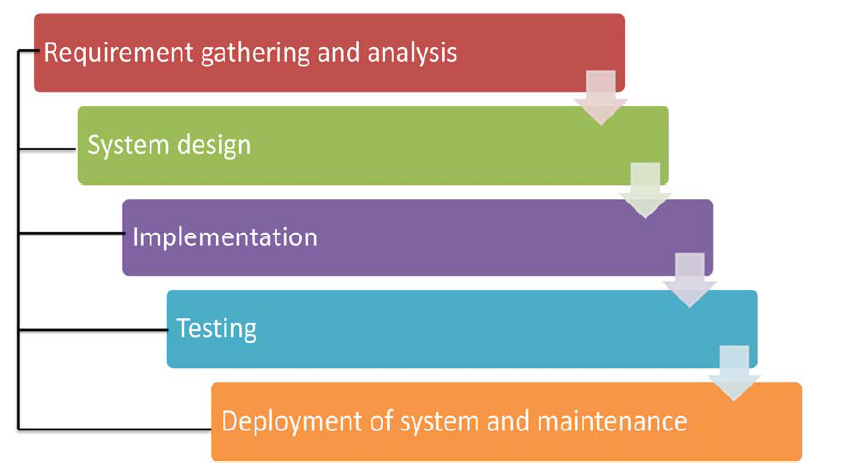
\includegraphics[width=10cm, height=5 cm]{"figures/waterfall.png"}
			\caption {Metoda Waterfall}\label{fig:one}
			\caption*{Sursa: Op.cit Marian STOICA }
		\end{figure}

	\quad În dezvoltarea agilă se îmbunătățește iterativ software-ul utilizând feedback-ul clienților pentru a converge către soluții. In loc de un singur model de proces mare implementat în SDLC convențional, ciclul de viață al dezvoltării este împărțit în părți mai mici, numite "incrementări" sau "iterații". Fiecare dintre aceste incrementări abordează fiecare dintre fazele convenționale de dezvoltare, iar apoi planificate si organizate intr-o perioada de timp fixa stabilita de client si echipa numita sprint (vezi figura \ref{fig:two}). Metodele au fost dezvoltate pentru a oferi o satisfacție mai mare clienților, pentru a scurta ciclul de viață al dezvoltării, pentru a reduce ratele de erori și pentru a se adapta cerințelor de afaceri care se schimbă pe parcursul procesului de dezvoltare. \footnote{ibidem}

\begin{figure}[!htb]
			\centering
			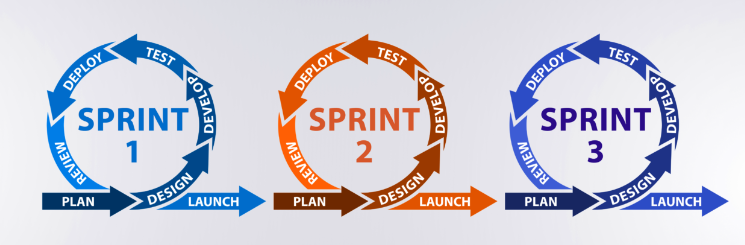
\includegraphics[width=14cm, height=4cm]{"figures/sprint.png"}
			\caption {Metoda Agile}\label{fig:two}
			\caption*{Sursa: John Adam, What is Agile software development?,2022, https://kruschecompany.com/agile-software-development/, accesat la data de 01.06.2023}
		\end{figure}

	\quad\quad Avand in vedere modul in care functioneaza o echipa din domeniul software putem deduce ca  exista diferențe semnificative dintre echipele clasice de lucru și echipele de dezvoltare software. Astfel, in urmatoarele randuri vom analiza ce elemente mai sunt diferite in activitatea lor:

\begin {itemize}

	\item \textbf{Abordarea față de munca în echipă}: Echipele clasice de lucru urmează o abordare liniară și secvențială a muncii în care etapele proiectului sunt finalizate în ordine, începând cu faza de planificare și continuând cu fazele de proiectare, dezvoltare, testare și implementare. În schimb, echipele de dezvoltare software folosesc o abordare iterativă, care implică cicluri scurte și repetate de dezvoltare, testare și feedback, în care mai multe etape ale proiectului sunt lucrate simultan.


	\item \textbf{Structura echipei}: În echipele clasice, membrii echipei sunt organizați în mod ierarhic, cu manageri și lideri de echipă care stabilesc obiectivele și sarcinile și care distribuie responsabilitățile în funcție de rolurile și competențele fiecăruia. În schimb, echipele de dezvoltare software sunt mai transversale, cu membrii ai echipei care dețin diverse abilități și cunoștințe tehnice, fiind implicați în toate aspectele proiectului. Aceste echipe se bazează pe colaborare și comunicare deschisă, în loc să se bazeze pe o ierarhie rigidă și o distribuție strictă a sarcinilor.

	\item \textbf{Luarea deciziilor}: În echipele clasice, deciziile sunt luate în mod obișnuit de către manageri și liderii de echipă, care stabilesc direcția și planurile de acțiune și apoi le comunică membrilor echipei. În schimb, echipele de dezvoltare software au o abordare mai colaborativă în luarea deciziilor, în care membrii echipei își aduc contribuția și împărtășesc feedback-ul și împreună ajung la un consens în luarea deciziilor.

	\item\textbf{Managementul proiectelor}: În echipele clasice, managementul proiectelor este adesea o abordare de sus în jos, cu managerii care planifică și organizează activitățile și atribuie sarcini membrilor echipei. În schimb, echipele de dezvoltare software folosesc adesea metodologii agile, cum ar fi Scrum sau Kanban, care implică un management colaborativ și iterativ al proiectelor. Acest lucru înseamnă că membrii echipei împărtășesc responsabilitatea pentru planificarea, dezvoltarea și testarea proiectului, și sunt în mod constant în căutarea de feedback-ul utilizatorilor pentru a îmbunătăți produsul.

	\item \textbf{ Instrumente și tehnologii}: Echipele clasice folosesc adesea instrumente și tehnologii tradiționale de management de proiect, cum ar fi tabele și software pentru planificare și urmărire. În timp ce echipele de dezvoltare software folosesc adesea instrumente de colaborare online, cum ar fi platforme de gestionare a codului sursă, de gestionare a sarcinilor și de comunicație. Aceste instrumente permit o colaborare mai eficientă și o urmărire mai precisă a progresului proiectului.

	\item De asemenea, în echipele de dezvoltare software, este comun să se utilizeze \textbf{practici de dezvoltare software} precum testarea automatizată, integrarea continuă și livrarea continuă. Aceste practici permit o dezvoltare mai rapidă și o livrare mai frecventă a funcționalităților către utilizatori, iar feedback-ul utilizatorilor poate fi integrat rapid în procesul de dezvoltare.

	\item În ceea ce privește \textbf{comunicarea}, echipele clasice tind să aibă o comunicare mai formală și structurată, în timp ce echipele de dezvoltare software au o comunicare mai deschisă și transparentă. Comunicarea este esențială în ceea ce privește succesul unei echipe și a unui proiect, indiferent de abordarea de lucru adoptată.

	\end{itemize}
	

	\quad Este important de mentionat si rolurile posibile pe care le ocupa membrii echipei pe perioada unui proiect. Există o varietate de roluri într-o echipă de dezvoltare software, fiecare cu responsabilități specifice pentru a ajuta la crearea și livrarea cu succes a unui produs software de înaltă calitate. Fiecare rol într-o echipă de dezvoltare software are propriile sale responsabilități și contribuții specifice la crearea și livrarea unui produs software de succes.  Iată câteva dintre cele mai comune roluri într-o astfel de echipă:

\begin{itemize}
	\item \textbf{Software Engineer :} este membrul echipei care este responsabil de scrierea codului pentru a crea și implementa funcționalitatea software-ului. Dezvoltatorul software ar trebui să aibă o bună înțelegere a limbajelor de programare și a arhitecturii software-ului. Printre limbajele de programare comune utilizate în dezvoltarea de software se numără Java, Python, C++, JavaScript, Ruby și altele.\footnote{Matt Warcholinski, 7 Crucial Roles in a Successful Software Development Team, https://brainhub.eu/library/crucial-roles-in-software-development-team, accesat in data de 01.06.2023}

	\item \textbf{Business Analyst} într-o echipă de dezvoltare software este de a analiza nevoile de afaceri ale clienților și de a traduce aceste nevoi în cerințe funcționale pentru dezvoltarea software. Ei lucrează strâns cu clienții și cu membrii echipei de dezvoltare pentru a se asigura că software-ul dezvoltat îndeplinește cu succes nevoile și cerințele afacerii.\footnote{ibidem}

	\item \textbf{ Tester-ul software/Inginer QA:}are rolul de a testa și verifica funcționalitatea software-ului pentru a asigura că îndeplinește cerințele și standardele de calitate specificate. Testerii software trebuie să aibă o bună înțelegere a procesului de testare și a tehnicilor de testare, precum și a automatizării testelor.\footnote{ibidem}

	\item \textbf{ Managerul de proiect:}  este responsabil de supervizarea proiectului de dezvoltare software, inclusiv gestionarea echipei, crearea planurilor de proiect și asigurarea că proiectul este finalizat la timp și în bugetul alocat. Managerii de proiect trebuie să aibă o bună înțelegere a metodologiilor de dezvoltare software și a procesului de gestionare a proiectelor.\footnote{Victoria Shashkina, Software development team structure: deciding factors, approaches, roles, and responsibilities, 2022, https://itrexgroup.com/blog/software-development-team-structure/, accesat la data de 01.06.2023}

	\item\textbf{Product Owner} are responsabilitatea de a defini și prioritiza lista de activități (backlog-ul) ale produsului, asigurându-se că sunt în concordanță cu nevoile părților interesate și obiectivele de afaceri. Ei acționează ca o punte între echipa de dezvoltare și clienți, conducând viziunea produsului și facilitând colaborarea.\footnote{ibidem}
	
	\item \textbf{Designerul UX/UI:} este responsabil pentru crearea designului de experiență și interfață pentru produsul software. Acesta trebuie să aibă o bună înțelegere a nevoilor și preferințelor utilizatorului final și să poată crea interfețe atractive, intuitive și eficiente.\footnote{ibidem}

	\item\textbf{Inginer DevOps:}  este responsabil pentru procesul de dezvoltare software, inclusiv dezvoltarea, testarea și implementarea aplicațiilor software. Inginerii DevOps trebuie să aibă o bună înțelegere a infrastructurii IT și a tehnicilor de automatizare a dezvoltării software.\footnote{ibidem}

	\item \textbf{Scrum Master} este responsabil de implementarea și facilitarea metodologiei Scrum într-o echipă de dezvoltare software. Ei asigură că membrii echipei urmează framework-ul agil și că proiectele sunt finalizate la timp și în cadrul bugetului. De asemenea, acționează ca mediator între echipa de dezvoltare și părțile interesate, ajutând la rezolvarea oricăror probleme care pot apărea.\footnote { Sergey Ovcharenko, 10 Key Roles in a Software Development Team: Who is Responsible for What?,https://alcor-bpo.com/recruitment-news/10-key-roles-in-a-software-development-team-who-is-responsible-for-what/, accesat in data de 01.06.2023}

	\item \textbf{ Software Architect} este responsabil pentru proiectarea arhitecturii software și a soluțiilor tehnice care să răspundă nevoilor de afaceri și cerințelor tehnice ale proiectului. El colaborează cu membrii echipei de dezvoltare software pentru a asigura că soluția lor este în conformitate cu standardele și practicile bune, și că este scalabilă și ușor de întreținut. Arhitectul de soluții acționează ca un lider tehnic și un consultant pentru echipa de dezvoltare software, oferind îndrumare și asistență în proiectarea și dezvoltarea software-ului.\footnote{ibidem}

	\item \textbf{Tech Lead-ul} este un programator cu experiență responsabil de sarcinile tehnice, precum revizuirea codului și mentoratul programatorilor. Liderii de echipă prioritizează și organizează procesul de lucru, menținând conexiuni între echipe și îmbunătățind motivația și moralul echipei. Aceste roluri sunt despre a fi lideri din perspective diferite în dezvoltarea software.
\footnote{ibidem}


	\subsection {Beneficiul implicarii team members – studiu de caz }
	
	
	\quad\quad  In contextul actual al dezvoltarii conducerii echipelor, s-a evidentiat o tot mai mare atentie asupra importantei implicarii membrilor echipei in acest proces. Desi exista diverse articole si informatii despre team leaders si leadership, relativ putine au explorat impactul implicarii membrilor echipei in procesul de formare si dezvoltare a unui team leader. 

	\quad Un articol in aceasta directie este a lui Paul Lyons, care isi propune prin lucrarea sa "Team member involvement in team leader training and performance", sa afle daca membrii echipei pot să ofere și chiar să modeleze, variabile de îmbunătățire a performanței care pot ajuta un lider de echipă sau un supervizor să acționeze mai eficient în beneficiul echipei și al organizației.\footnote{Paul Lyons, Team member involvement in team leader training and performance, 2006}.  Prin utilizarea grupurilor de discuții și a metodei Q-sort, a reusit sa implice membrii unei echipe in identificarea elementelor practice de performanță legate de comportamentul liderilor lor de echipă .Integrând aceste elemente de performanță în designul instruirii pentru liderii de echipă și utilizând Skills Chart ca instrument de instruire, s-au putut compara două grupuri de lideri de echipă: un grup (grupul de studiu) ale cărui instruiri s-au concentrat, în mod specific, pe elementele de performanță generate de echipă și alt grup (grupul tradițional) ale cărui instruiri s-au concentrat pe elementele generale de performanță ale liderilor de echipă. 

	\quad In urma rezultatelor obtinute in cadrul acestui studiu, s-a constatat că implicarea membrilor echipei în procesul de formare și crearea de procese de învățare prin acțiune au avut un impact pozitiv asupra performanței grupurilor cooperative. De asemenea, a fost evidențiată importanța directă a membrilor echipei în identificarea și specificarea comportamentelor critice ale liderilor de echipă, în sprijinul performanței membrilor echipei, ca fiind o formă de autonomizare. 

	\quad În concluzie, rezultatele acestui studiu au subliniat relevanța dezvoltării abilităților liderilor de echipă și a impactului acestora asupra performanței echipei, contribuind la obținerea unui avantaj competitiv în cadrul organizației. Astfel, acest articol subliniaza inca o data importanta pe care o au membrii echipei in atingerea obiectivelor atat la nivel de echipa cat si la nivel de organizatie  si evidentiaza nevoia de a le acorda o atentie sporita pe viitor.



\newpage
\end{itemize}

\setcounter{section}{2}
	\section{Studiu de caz }

	\quad\quad Prin acest capitol se urmărește identificarea acelor abilitati ce sunt  considerate importante unui team leader pentru a putea obtine succesul organizatiei din care face parte. De asemenea, acest capitol reprezintă partea practică a prezentei lucrări de disertatie și are rolul de a determina diferentele dintre perspectiva membrilor echipei si a team leader-ului privind  aceste abilitati. Datele colectate și rezultatele obținute în urmă prelucrării și interpretării constituie baza pentru organizațiile care doresc să creeze programe pentru dezvoltarea abilitatilor ce sunt necesare unui team leader in diverse contexte actuale.

	\subsection{Scop si obiective}

	\subsection{Metodologia cercetarii}
		\subsubsection{Metoda Cercetarii}
	\qquad\space Pentru a atinge scopul cercetării și pentru a obține informațiile necesare unei analize cât mai complexe și cât mai detaliate cu referire la tema abordată în această lucrare, am optat pentru o metodă de cercetare cantitativă în locul unei cercetări calitative.
	\quad Metodă cantitativă pe care am folosit-o în cercetare a fost sondajul de opinie, care este o metodă indirectă de colecatare a datelor. Că și instrument al sondajului de opinie am folosit chestionarul.\footnote{Sandor Dan Sorin, \textit{Metode și Tehnici de Cercetare în Științele Sociale}, 2013, p.133,145}
		\subsubsection{Profilul respondentilor}
	\quad Profilul stabilit al respondenților pentru cercetarea primară cantitativă a fost angajat al firmei A care lucreaza in domeniul IT, care are  o experienta profesionala de minim 6 luni, din România.Am ales să obțin răspunsurile de la angajații acestei companii pentru a obține o perspectivă specifică a organizației în ansamblul său, pe care toți angajații o împărtășesc.
		\subsubsection{Instrumentul cercetarii}
	\quad Chestionarul (vezi Anexa 1) a fost lansat online cu ajutorul platformei Google Forms și a fost promovat  pe diverse grupuri din interiorul firmei A. Astfel, orice angajat putea completă chestionarul online, iar odată completat acesta intra direct în baza de date. Această tehnică este una destul de rapidă deoarece chestionarul durează 3-5minute maxim pentru a-l completa și nu implică costuri deoarece Google Forms este o platforma gratuită.

	\subsection{Analiza si interpretarea datelor}

	\quad Datele culese din sondajul de opinie au fost culese cu ajutorul unui chestionar (vezi Anexa 1), lansat online, în perioada 20 mai- 10 iunie 2023. Pentru lansarea chestionarului am folosit aplicația Google Forms. Avantajul utilizării acestei aplicații constă în faptul că răspunsurile primite sunt centralizate și prelucrate în mod automat. Un alt avantaj al utilizării Google Forms că mijloc de a distribui un sondaj constă în generarea automată de grafice pe baza răspunsurilor primite. 

	\subsection{ Concluzii- studiu de caz}

\newpage
\setcounter{section}{3}
	\section{Concluzii}	






	
	







\newpage

	\section*{Referințe bibliografice}
	\addcontentsline{toc}{section}{\textsc{Referințe bibliografice}}
	\space
	\bigskip
	\bigskip

	\textbf{Cărți în format electronic:}
	

	\textbf{Articole științifice în format electronic:}
	\begin{enumerate}[1.]
		\item Frederick P. Morgeson, D. Scott DeRue, Elizabeth P. Karam, Leadership in Teams: A Functional Approach to Understanding Leadership Structures and Processes,2010
	\end{enumerate}

	\textbf{Articole preluate de pe pagini web:}












\end{document}